\newpage

Algorytm HALS jest najbardziej złożony z trzech wykorzystanych w zadaniu algorytmów. Dlatego w jego głównej pętli są tworzone zmienne pomocnicze, które swoimi nazwami przypominają oznaczenia w formule matematycznej algorytmu. Wygląda ona w następujący sposób:

\begin{figure}[H]
	\centering
	%\hspace*{-1in}
	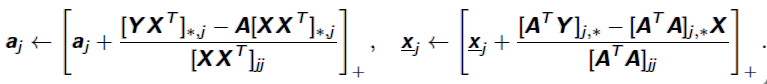
\includegraphics[scale = 0.5]{hals_wzor.png} 
	\label{rys:hals_wzor} 
\end{figure}

Jak widać na poniższym listingu, implementacja HALS zawiera dwie pętle. Dzieje się tak dlatego, że podczas jednego przebiegu pętli wewnętrznej zostaje zmieniona tylko jedna kolumna w macierzy \textit{A} i jeden wiersz w macierzy \textit{X}. Żeby całe macierze przeszły ten proces, pętla od 1 do \textit{J} musi wykonać się w całości. Z tego powodu normalizacja zostaje wykonana dopiero po pełnym przebiegu pętli wewnętrznej, a następnie obliczany jest błąd residualny znormalizowanych macierzy.

\vspace{5mm}
\begin{minipage}{\linewidth}
\begin{lstlisting}[linewidth=14.5cm]
%% Algorytm HALS
%% Inicjalizacja
A_hals = rand(size(Y,1), J);
X_hals = rand(J, size(Y,2));

%% Update
MaxIter = 400;
res_hals = zeros(1,MaxIter);

for k = 1: MaxIter
	% Inicjalizacja zmiennych pomocniczych
	XXT = X_hals*X_hals';
	YXT = Y*X_hals';
	ATA = A_hals'*A_hals;
	ATY = A_hals'*Y;
	
	for j = 1 : J
	% Update A       
	nextA = A_hals(:,j) 
		+ (YXT(:,j) - A_hals*XXT(:,j))./max(eps,XXT(j,j));
	A_hals(:, j) = max(0, nextA);  
	
	% Update X
	nextX = X_hals(j,:) 
		+ (ATY(j,:) - ATA(j,:)*X_hals)./max(eps,ATA(j,j));
	X_hals(j, :) = max(0, nextX);       
	end

	% Normalizacja
	A_hals = A_hals*(diag(1./max(eps, sum(A_hals, 1))));
	
	% Blad residualny
	res_hals(k) = norm(Y - A_hals*X_hals, 'fro')/norm(Y, 'fro');
end
\end{lstlisting}
\end{minipage}